


\tikzset{every picture/.style={line width=0.75pt}} %set default line width to 0.75pt        

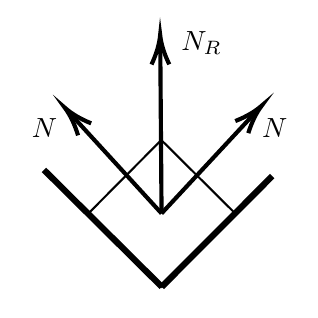
\begin{tikzpicture}[x=0.75pt,y=0.75pt,yscale=-1,xscale=1]
%uncomment if require: \path (0,307); %set diagram left start at 0, and has height of 307

%Shape: Square [id:dp11158416935531834] 
\draw   (293.64,158.12) -- (328.88,122.64) -- (364.36,157.88) -- (329.12,193.36) -- cycle ;
%Straight Lines [id:da5782322433552698] 
\draw [line width=2.25]    (272.33,137) -- (329.12,193.36) ;
%Straight Lines [id:da31004030039107744] 
\draw [line width=2.25]    (329.12,193.36) -- (382.33,140) ;
%Straight Lines [id:da7515473055819413] 
\draw [line width=1.5]    (329,158) -- (375.29,108.2) ;
\draw [shift={(377.33,106)}, rotate = 132.91] [color={rgb, 255:red, 0; green, 0; blue, 0 }  ][line width=1.5]    (14.21,-4.28) .. controls (9.04,-1.82) and (4.3,-0.39) .. (0,0) .. controls (4.3,0.39) and (9.04,1.82) .. (14.21,4.28)   ;
%Straight Lines [id:da17146564901097117] 
\draw [line width=1.5]    (329,158) -- (284.36,109.21) ;
\draw [shift={(282.33,107)}, rotate = 47.54] [color={rgb, 255:red, 0; green, 0; blue, 0 }  ][line width=1.5]    (14.21,-4.28) .. controls (9.04,-1.82) and (4.3,-0.39) .. (0,0) .. controls (4.3,0.39) and (9.04,1.82) .. (14.21,4.28)   ;
%Straight Lines [id:da34529906812085653] 
\draw [line width=1.5]    (329,158) -- (328.36,75) ;
\draw [shift={(328.33,72)}, rotate = 89.56] [color={rgb, 255:red, 0; green, 0; blue, 0 }  ][line width=1.5]    (14.21,-4.28) .. controls (9.04,-1.82) and (4.3,-0.39) .. (0,0) .. controls (4.3,0.39) and (9.04,1.82) .. (14.21,4.28)   ;

% Text Node
\draw (265,111) node [anchor=north west][inner sep=0.75pt]    {$N$};
% Text Node
\draw (376,111) node [anchor=north west][inner sep=0.75pt]    {$N$};
% Text Node
\draw (337,69) node [anchor=north west][inner sep=0.75pt]    {$N_{R}$};


\end{tikzpicture}
